% This is "sig-alternate.tex" V2.0 May 2012
% This file should be compiled with V2.5 of "sig-alternate.cls" May 2012
%
% This example file demonstrates the use of the 'sig-alternate.cls'
% V2.5 LaTeX2e document class file. It is for those submitting
% articles to ACM Conference Proceedings WHO DO NOT WISH TO
% STRICTLY ADHERE TO THE SIGS (PUBS-BOARD-ENDORSED) STYLE.
% The 'sig-alternate.cls' file will produce a similar-looking,
% albeit, 'tighter' paper resulting in, invariably, fewer pages.
%
% ----------------------------------------------------------------------------------------------------------------
% This .tex file (and associated .cls V2.5) produces:
%       1) The Permission Statement
%       2) The Conference (location) Info information
%       3) The Copyright Line with ACM data
%       4) NO page numbers
%
% as against the acm_proc_article-sp.cls file which
% DOES NOT produce 1) thru' 3) above.
%
% Using 'sig-alternate.cls' you have control, however, from within
% the source .tex file, over both the CopyrightYear
% (defaulted to 200X) and the ACM Copyright Data
% (defaulted to X-XXXXX-XX-X/XX/XX).
% e.g.
% \CopyrightYear{2007} will cause 2007 to appear in the copyright line.
% \crdata{0-12345-67-8/90/12} will cause 0-12345-67-8/90/12 to appear in the copyright line.
%
% ---------------------------------------------------------------------------------------------------------------
% This .tex source is an example which *does* use
% the .bib file (from which the .bbl file % is produced).
% REMEMBER HOWEVER: After having produced the .bbl file,
% and prior to final submission, you *NEED* to 'insert'
% your .bbl file into your source .tex file so as to provide
% ONE 'self-contained' source file.
%
% ================= IF YOU HAVE QUESTIONS =======================
% Questions regarding the SIGS styles, SIGS policies and
% procedures, Conferences etc. should be sent to
% Adrienne Griscti (griscti@acm.org)
%
% Technical questions _only_ to
% Gerald Murray (murray@hq.acm.org)
% ===============================================================
%
% For tracking purposes - this is V2.0 - May 2012

\documentclass{sig-alternate}

\pagenumbering{arabic}

\usepackage{array}
\usepackage{enumitem}
\usepackage{float}


\begin{document}
%
% --- Author Metadata here ---
\conferenceinfo{CS846}{'15 Waterloo, Canada}
\CopyrightYear{2015} % Allows default copyright year (20XX) to be over-ridden - IF NEED BE.
%\crdata{0-12345-67-8/90/01}  % Allows default copyright data (0-89791-88-6/97/05) to be over-ridden - IF NEED BE.
% --- End of Author Metadata ---

\title{CodeSketch: Drawing Diagrams in Source Code} 

\numberofauthors{2}

\author{
\alignauthor
Reza Adhitya Saputra\\
       \affaddr{University of Waterloo}\\
       \email{radhitya@uwaterloo.ca}
% 2nd. author
\alignauthor
Raminder Sodhi\\
       \affaddr{University of Waterloo}\\
       \email{rjsodhi@uwaterloo.ca}
}


\maketitle
\begin{abstract}
\label{abstract}


A picture is worth a thousand words. Similarly, software developers sketch diagrams for various purposes.  The diagrams they draw can be flowcharts, architecture diagrams, or algorithm descriptions. We develop a tool called CodeSketch based on diagramming practice in Open Source Software (OSS) development. Using CodeSketch, a developer can draw a diagram consists of rectangles, lines, arrows, and texts. The tool then converts the diagram to ASCII art which is directly embedded in source code. Compared to other diagram representation, created diagrams using CodeSketch can coexist with source code files, they do not require specific graphics viewer tool other than a text editor, and they are easy to be stored in a revision control system. Finally, we conduct a user study where participants can use our tool followed by collecting their feedback.

\end{abstract}

%% A category with the (minimum) three required fields
%\category{H.4}{Information Systems Applications}{Miscellaneous}
%%A category including the fourth, optional field follows...
%\category{D.2.8}{Software Engineering}{Metrics}[complexity measures, performance measures]
%
%\terms{Theory}

\keywords{Source code comments, documentation, diagrams, ASCII art}

\section{Introduction}
\label{introduction}

Diagrams are important visual representation which are widely used in design arts, engineering, and science. The use of diagrams and images is also pervasive in software development since diagrams are viewed as alternatives to verbal communication. Furthermore, diagrams enables developers to visualize concepts and communicate ideas. For example, a developer would doodle diagrams on scrap papers or whiteboards during a discussion with their coworkers. In more formal purposes, diagrams can be created using a specific designer tool. However, the designer tool restricts the developer to use a particular framework so the created diagrams cannot be exported easily to other platforms with different development tools.

In co-located software development, diagrams are used during discussions, meetings, or presentations. However, these diagrams have transitory nature \cite{Cherubini2007}. One reason is that because they only serve a purpose to explain concepts to coworkers. After the coworkers understood, sketches on whiteboard will be erased and diagrams on scrap papers would be thrown into garbage bins. Although these diagrams can be converted digitally for long term purposes, such as code documentation, redrawing these diagrams is wearisome. 

In Open Source Software (OSS) development, developers avoid creating a lot of bitmap-based diagrams on documentation or wiki pages. This is because they do not bother to keep these diagrams be updated when they changed their source code \cite{Yatani2009}. Nevertheless, if they must draw diagrams to communicate their ideas, they tend to use ASCII art. Although ASCII art is a simple form of diagrams, it has a practical benefit compared to other graphical representations: ASCII art enables developers not to depend on a specific graphical tool. Furthermore, in an open source project every developer may not use the same tools. Therefore, a tool-independent diagram representation is required. 

This project focuses on OSS settings and the use of ASCII art. We developed a diagramming tool to create ASCII art based on criteria we have collected during literature study. The created diagrams can be edited easily and viewed without a specific tools. We did a user study conducted on (X) participants. The user study consists of a number of exercises on which participants can try to use our tool, then followed with questionnaire. As a final step, we gather their interesting feedback.



\section{Related Work}
\label{related_work}

Our proposed idea is related to why developers draw diagrams and creating diagrams as source code comments.

\textbf{Why developers draw diagrams}. In co-located teams, diagrams help developers to understand source code, starting discussions, improve documentations and they can be used as presentation aids during a meeting \cite{Cherubini2007}.  In OSS community, developers agree that diagramming is useful but they do not like to redraw diagrams after they updated their source code  \cite{Yatani2009, Eunyoung2010}. If they must draw diagrams, they tend to use ASCII art since they have low cost in creation. Moreover, they prefer to put diagrams inside a revision control system, so everyone can keep track changes. In another study, the use of ASCII art in bug reports also has been observed \cite{Twidale2005}.

\textbf{Creating diagrams as source code comments}. GUIIO is a tool to create a GUI mockup embedded in source code \cite{Simpson2011}. Similar to our tool, they also use ASCII art. The mockup is used as an explanation to source code snippets which actually implement the actual GUI. They argue that the approach can reduce window switching between source code and designer tool. However, GUIIO cannot be used to draw more general diagrams, e.g, flowcharts.

\section{System Design}
\label{system_design}

We summarize nine criteria of an ideal diagramming tool based on literature study of previous research of diagramming practice in OSS development  \cite{Yatani2009, Eunyoung2010}. 
Subsequently, table \ref{codesketch_design_decision} shows the design decision of CodeSketch based on these criteria. Note that CodeSketch does not satisfies all criteria.

\begin{enumerate} [nolistsep]
\item Diagrams coexist with existing communication tools. 
\item The diagramming tool is widely available and free. 
\item Diagrams can be easily published based on who the intended audience is. 
\item The diagramming tool can be easily integrated into development infrastructure.
\item Diagrams are easily to be stored in a revision control system. 
\item The "source code" of diagrams can be shared, for example XML-like language for GUI design. 
\item Diagrams are  not tedious to create and edit (Possibly fully automated).
\item Diagrams do not require specific tools to create and display. 
\item A change of a diagram can be observed, similar to diff tool

\end{enumerate}

\begin{table}[h]
\scriptsize
\begin{tabular}{|p{55px}|p{170px}|}
\hline
\textbf{Criteria - 
Supportability} & \textbf{Design Decision} \\ \hline

1 - Yes & 
Diagrams created using CodeSketch should be easily embedded into various text-based communication tools, such as mailing list, IRC, bug reports, and code review tools. Because the diagrams are text-based, this criteria can be fulfilled.
\\ \hline

2 - Yes & 
We design CodeSketch as a plugin for Github to be a free web-based app.
\\ \hline

3 - No & 
We represent diagrams with unicode characters, so we cannot satisfy this criteria. For example, yhe diagrams are sufficient enough for explaining code to coworkers, but unsuitable for a formal meeting e.g. with stakeholders or end users.
\\ \hline

4 - Yes & 
We implement CodeSketch as a web based tool and will be embedded as source code comment, so it is platform independent. 
\\ \hline

5 - Yes & 
Our diagrams are text-based. Unlike binary images, they are compatible with any revision control system.
\\ \hline

6 - Yes & 
The diagrams themselves are source code composed of Unicode characters. 
\\ \hline

7 - No & 
An ambitious goal is to automate the creation of diagrams. However, our tool is not designed to encourage developers draw more diagrams or to make diagramming easier. 
\\ \hline

8 - Partially & 
ASCII diagrams require a specific tool to be created, since manually placing every character would be cumbersome. However our diagrams can be viewed without using a specific viewer tool.
\\ \hline

9 - No & 
Diff tool can be used to compare two ASCII diagrams. However, diff tool is line based so  a single character editing will highlight an entire line. 
\\ \hline

\end{tabular}
\caption {CodeSketch's design decision}
\label{codesketch_design_decision}
\end{table}



\section{Implementation}
\label{implementation}

\begin{figure}
\centering
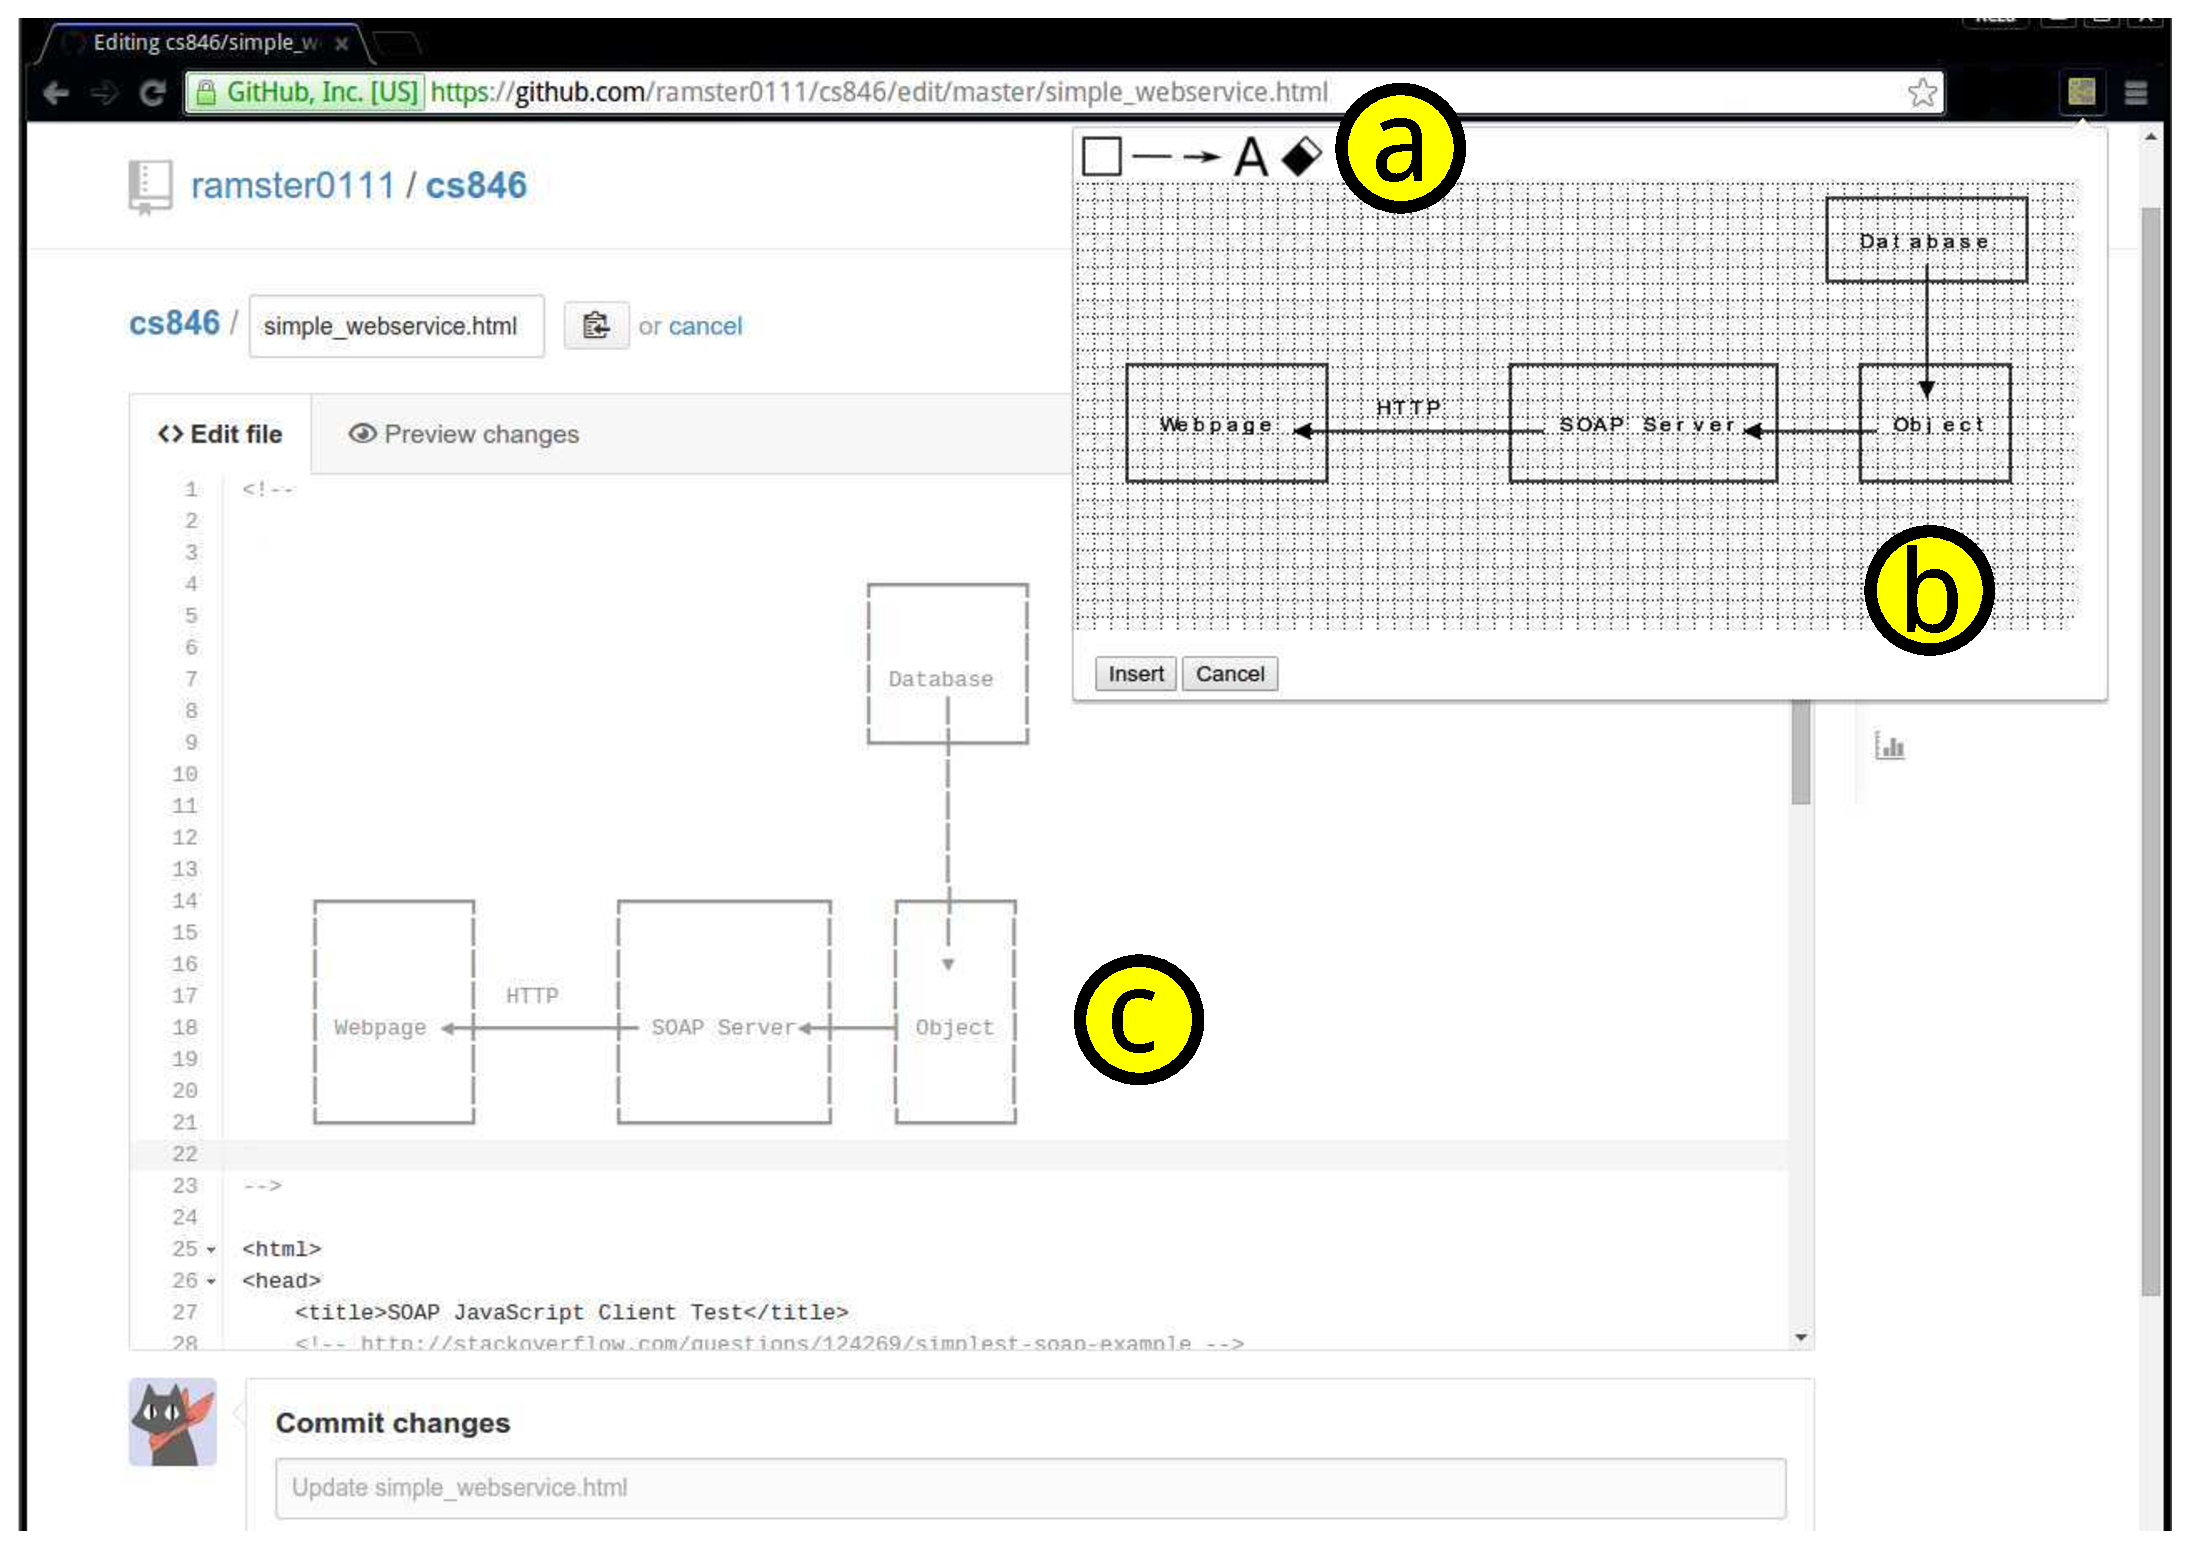
\includegraphics[scale=.23]{codesketch_screenshot.eps}
\caption{CodeSketch Interface. (a) a drawing toolbar. (b) a drawing canvas. (c) generated ASCII art as a HTML comment.}
\label{fig:codesketch_screenshoot}
\end{figure}


As can be seen in figure \ref{fig:codesketch_screenshoot} Our prototype of CodeSketch is a chrome extensions built using HTML5 canvas and Javascript. We provide a drawing canvas where the user can draw diagrams with the help of drawing tools likes rectangles, lines, arrow lines, text and eraser. The drawing diagram can then be embedded in ASCII format at  the current cursor position in GitHub code edit boxes. We also keep the UI to be simple to make the tool easier to use.


\section{Evaluation}
\label{evaluation}

To investigate diagrams in source code and answer our research questions, we designed a study in which participants were asked to draw diagrams using our tool for 4 different exercises and then answer a set of questions following it. In the beginning of the survey we gave participants time to get comfortable with the tool. Demonstrations of some basic patterns like loops was done so that the users are able to complete the tasks comfortably. The survey consisted of 3 drawing tasks and a comparison task. The drawing tasks consisted of drawing a diagram for linked list traversal, a class diagram and an architecture diagram for any system with which the users are most familiar with. The comparison task was a comparison between text based documentation and text + image based documentation.

\subsection{Drawing Task 1}
In this task the participants were presented with a simple link list traversal function and were asked to draw meaningful drawings. Majority of the participants gave importance to the data structure being used while some concentrated more on the input and output of the function.

\subsection{Drawing Task 2}
In this task the participants were asked to draw a class diagram for any scenario they want in the animal/plant kingdom. We noticed that the majority of the people concentrated more on relationships between the classes, little importance was given to member functions and members as such.

\subsection{Drawing Task 3}
In this task the participants were asked to draw system they know the most about. We observed that all the participants were successful in drawing basic interactions between the various components of  these system. The representations were clear and concise.

\subsection{Comparison Task}
For the comparison task the participants were asked their feedback on code understanding based on text based documentation against ASCII image based documentation. They were first ask to see the code and think loud about it, after going through the code they were asked to see the both the documentation and their feedback was taken. In general the feedback was that the image based documentation was helpful in visualizing the scenario better. The participants expressed that on just seeing the image they could get a general idea on what is happening in the code in comparison to textual documentation. 


\begin{figure}[H]
\centering
\includegraphics[scale=.35]{drawing_task_1.png}
\caption{Drawing Task 1 \textit{(drawn by P2)}}
\label{fig:drawing_task_1}
\end{figure}

\begin{figure}[H]
\centering
\includegraphics[scale=.35]{drawing_task_2.png}
\caption{Drawing Task 2 \textit{(drawn by P4)}}
\label{fig:drawing_task_2}
\end{figure}

\begin{figure}[H]
\centering
\includegraphics[scale=.35]{drawing_task_3.png}
\caption{Drawing Task 3 \textit{(drawn by P3)}}
\label{fig:drawing_task_3}
\end{figure}

\begin{figure}[H]
\centering
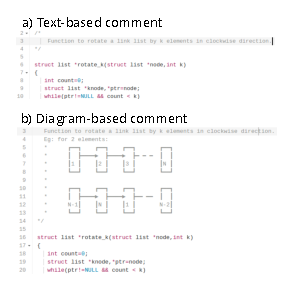
\includegraphics[scale=1.5]{comparison_task.eps}
\caption{Comparison Task}
\label{fig:comparison_task}
\end{figure}

\label{results}

\section{Discussion}

\section{Limitations and Future Work}

Although we receive positive feedback from participants about the use of CodeSketch, our evaluation does not answer how embedding diagrams improve code understanding. Therefore, we would like to know the effectiveness of embedding diagrams in various settings, for example, in code reviews and bug reports. When reviewing source code, developers have a problem in understanding code which they do not own. The lack of understanding makes them difficult to find defects on the source code \cite{Bacchelli2013}. A similar problem is also found in bug reports where reporters do not give much explanation \cite{Bettenburg2008}. We also would like to do comparison with a completely different approach  called Literate Programming \cite{Knuth1984}. In contrast to diagramming, literate programming also aims for code understanding through  incorporating compilable source code to literature writing.

Apart from code understanding, we also have several other future work in mind. First, we would like to investigate how can CodeSketch reduce task switching. Embedded diagrams in source code does not need window switching between code and diagrams, which is the design goal of CodePad \cite{Parnin2010}. Second, we feel that it is necessary to develop a way for easier diagramming. Ideally, editing and updating ASCII diagrams should not be cumbersome, or even fully automatic. Lastly, developing a customized diff tool to visualize how a diagram changes over time would be an interesting research direction. We envision the diff tool would be similar to Nonlinear Revision Control for Images \cite{Chen2011}. 


\section{Conclusions}


%ACKNOWLEDGMENTS are optional

%\section{Acknowledgments}
%Thanks for all the fish

\nocite{*}
\bibliographystyle{abbrv}
\bibliography{reference_846}  % sigproc.bib is the name of the Bibliography in this case

\end{document}
